\documentclass[12pt, a4paper]{article}
\usepackage[utf8]{inputenc}
\usepackage{physics}
\usepackage{graphicx}
\usepackage{amsmath}
\usepackage{cancel}
%code color
\usepackage{listings}
\usepackage{xcolor}

\definecolor{codegreen}{rgb}{0,0.6,0}
\definecolor{codegray}{rgb}{0.5,0.5,0.5}
\definecolor{codepurple}{rgb}{0.58,0,0.82}
\definecolor{backcolour}{rgb}{0.95,0.95,0.92}

\lstdefinestyle{mystyle}{
	backgroundcolor=\color{backcolour},   
	commentstyle=\color{codegreen},
	keywordstyle=\color{magenta},
	numberstyle=\tiny\color{codegray},
	stringstyle=\color{codepurple},
	basicstyle=\ttfamily\footnotesize,
	breakatwhitespace=false,         
	breaklines=true,                 
	captionpos=b,                    
	keepspaces=true,                 
	numbers=left,                    
	numbersep=5pt,                  
	showspaces=false,                
	showstringspaces=false,
	showtabs=false,                  
	tabsize=2
}

\lstset{style=mystyle}

\begin{document}
	\begin{center}
		Test 5: Spy Hunter Qubit (09/13/2021)
	\end{center}
	Mr. Phiphat Chomchit 630631028
	\begin{center}
		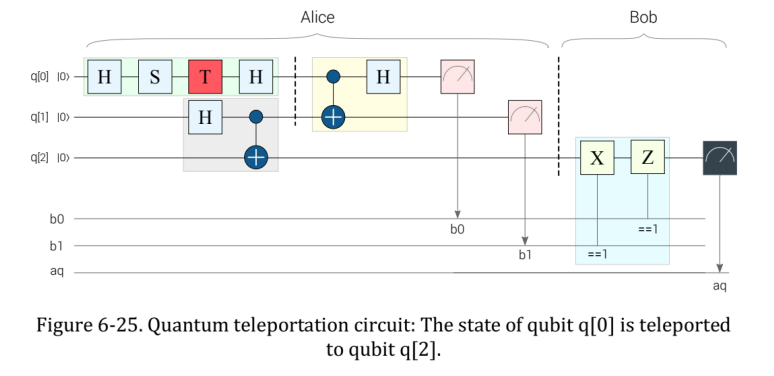
\includegraphics[scale=0.5]{problem.png}
	\end{center}
	\section{Have a spy}
	\begin{lstlisting}[language=Java, caption= Have  a spy]
		OPENQASM 2.0;
		include "qelib1.inc";
		//init bit and q-bit
		qreg alice[1];
		qreg connection[1];
		qreg bob[1];
		creg a1[1];
		creg a2[1];
		creg con[1];
		creg b1[2];
		creg b2[2];
		
		//Alice
		//Get two random bits
		reset alice[0];
		h alice[0];
		measure alice[0] -> a1[0];
		reset alice[0];
		h alice[0];
		measure alice[0] -> a2[0];
		reset alice[0];
		//set value
		if(a1==1) x alice[0];
		//apply hadamard
		if(a2==1) h alice[0];
		
		//spy
		swap  alice[0], connection[0];
		h connection[0];
		measure connection[0] -> con[0];
		reset connection[0];
		if (con==1) x connection[0];
		h connection[0];
		
		//Bob
		//random B1
		reset bob[0];
		h bob[0];
		measure bob[0] -> b1[0];
		
		//read q-bit
		swap connection[0], bob[0];
		if(b1==1) h bob[0];
		measure bob[0] -> b2[0];
		
	\end{lstlisting}
	
	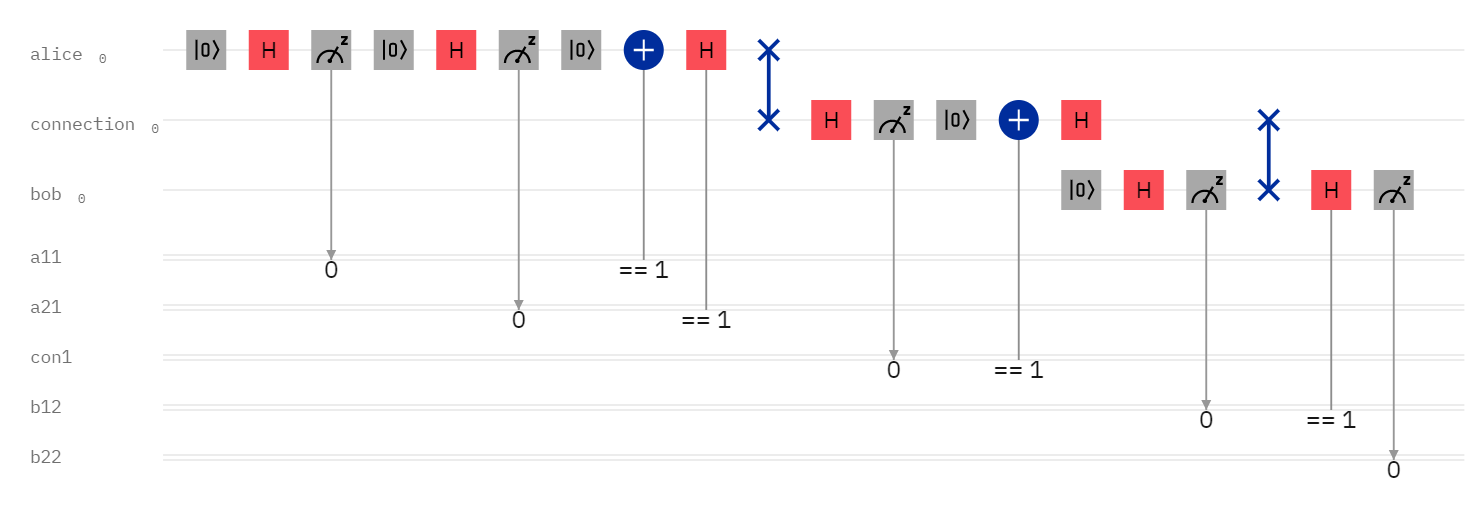
\includegraphics[scale=0.3]{circuit-ktk4pxiy.png}
	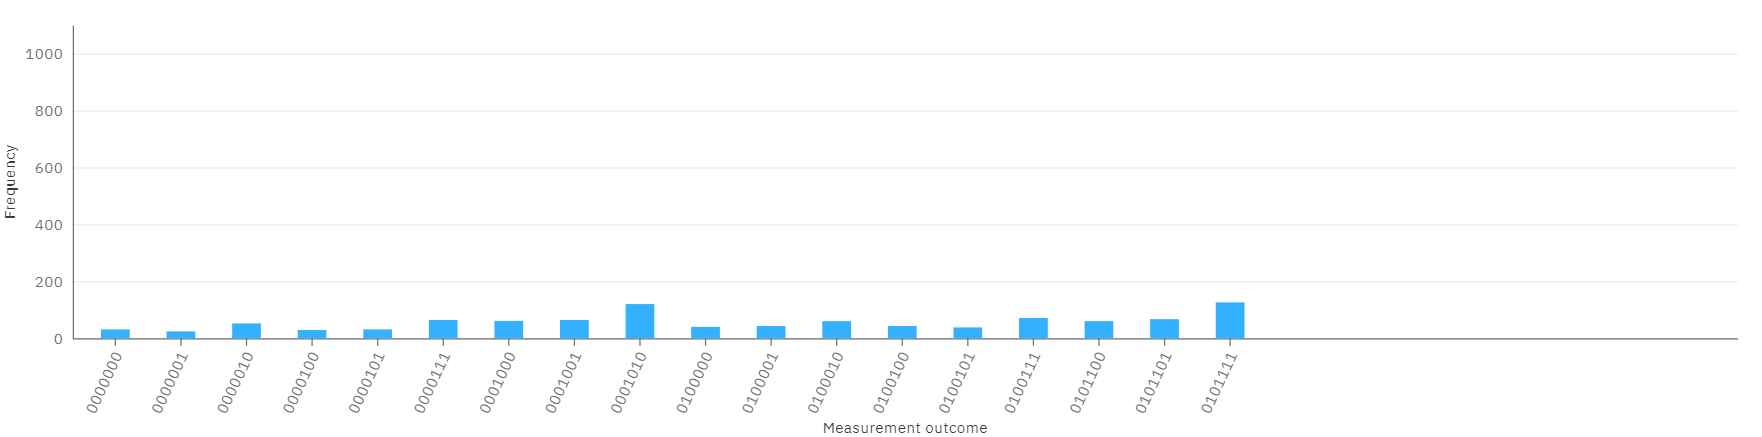
\includegraphics[scale=0.3]{bar-chart.png}
	\newpage
	\section{No spy}
	\begin{lstlisting}[language=Java, caption= No spy]
		OPENQASM 2.0;
		include "qelib1.inc";
		//init bit and q-bit
		qreg alice[1];
		qreg connection[1];
		qreg bob[1];
		creg a1[1];
		creg a2[1];
		creg con[1];
		creg b1[2];
		creg b2[2];
		
		//Alice 
		//add random bit
		reset alice[0];
		h alice[0];
		measure alice[0] -> a1[0];
		reset alice[0];
		h alice[0];
		measure alice[0] -> a2[0];
		reset alice[0];
		
		//set value
		if (a1==1) x alice[0];
		//apply hadamard
		if (a2==1) h alice[0];
		swap alice[0],connection[0];
		
		//Bob
		reset bob[0];
		h bob[0];
		measure bob[0] -> b1[0];
		swap connection[0],bob[0];
		if (b1==1) h bob[0];
		measure bob[0] -> b2[0];
	\end{lstlisting}
	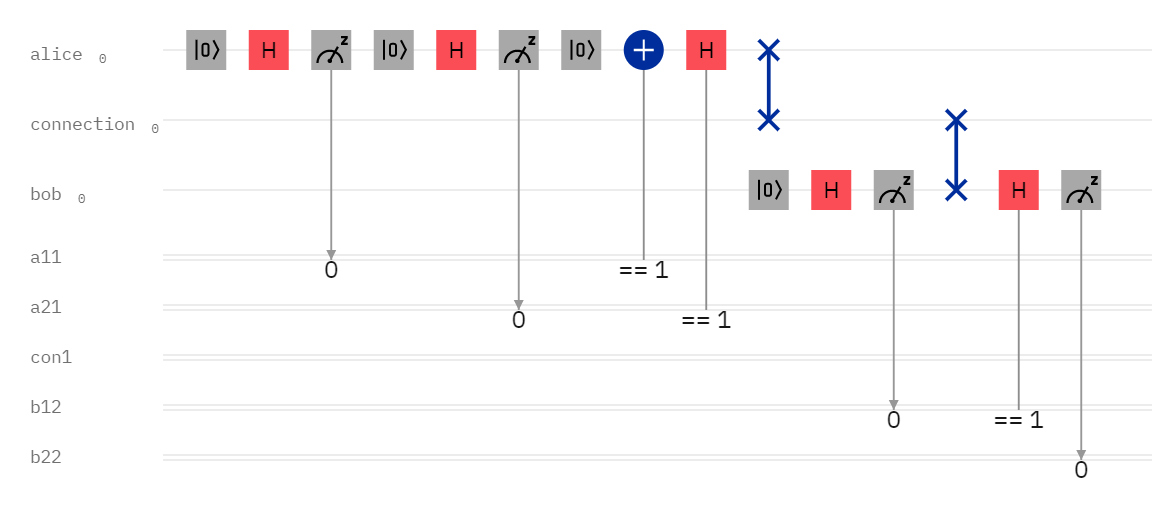
\includegraphics[scale=0.4]{circuit-ktkzgune.png}
	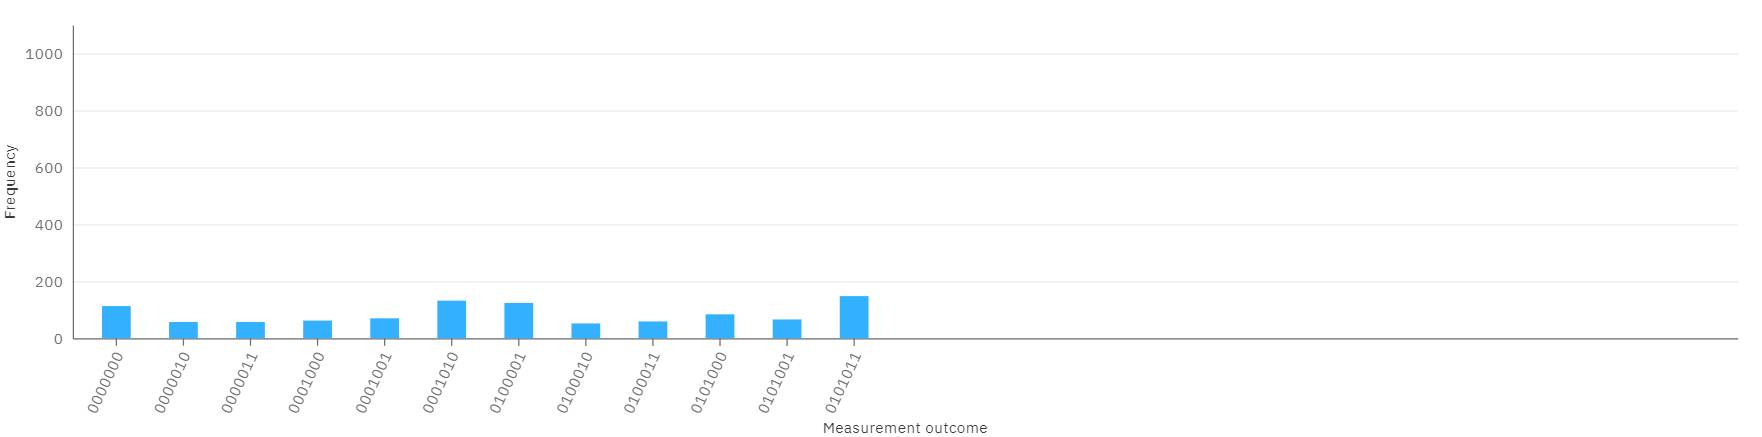
\includegraphics[scale=0.3]{bar-chart2.png}
\end{document}